\section{Kafka}

Kafka is a distributed, partitioned, replicated commit log service, that provides the functionality of a messaging system. It is used for collecting and delivering high volumes of data with low latency. Apache Kafka was originally developed by LinkedIn, and was subsequently open sourced in 2011. In 2012 Kafka became an Apache Top-Level Project.

The basic concepts of Kafka are the following:
\begin{itemize}
\item A \emph{topic} defines a stream of messages of a particular type.
\item A \emph{producer} is a process that publishes messages to a topic.
\item The published messages are stored at a cluster comprised of servers called \emph{brokers}. All coordination between the brokers is done through a Zookeeper cluster.
\item A \emph{consumer} is a process that subscribes to one or more topics and processes the feed of published messages.
\end{itemize}

\begin{figure}[H]
\centering
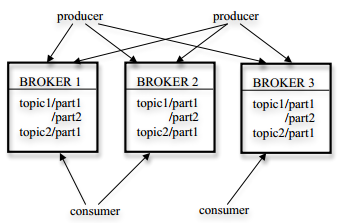
\includegraphics{figures/kafka_arch}
\caption{Kafka architecture}
\label{figure:kafka_arch}
\end{figure}

For each topic, the Kafka cluster maintains a partitioned log with the structure depicted on Figure \ref{figure:kafka_topic}. A \emph{partition} is essentially a commit log to which an ordered, immutable sequence of messages that is continually appended. Every message is assigned an offset: a sequential id number that uniquely identifies the message within the partition. Kafka only provides a total order over messages within a partition, not between different partitions in a topic.

\begin{figure}[H]
\centering
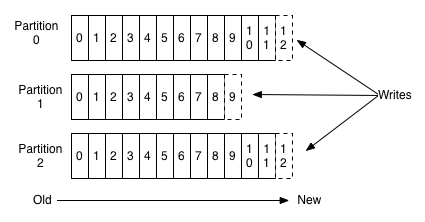
\includegraphics{figures/kafka_topic}
\caption{Kafka topic structure}
\label{figure:kafka_topic}
\end{figure}

All published messages remain stored at the brokers for a configurable period of time, whether or not they have been consumed. Kafka's performance is effectively constant with respect to data size, allowing a big volume of data to be retained. The only metadata retained for each consumer is the offset of the consumer in the log. By controlling this offset the consumer can read messages in any order. For example a consumer can advance its offset linearly as it reads messages or even reset to an older offset to reprocess them.

The partitions in the log serve several purposes. Firstly, they allow the log to scale in size, by being distributed over the brokers of the cluster. Moreover, the partitions are replicated across a configurable number of brokers to provide fault tolerance. For each partition one broker acts as the "leader",  handling all the requests for the partition, and zero or more brokers act as "followers", replicating the leader. Finally, partitions act as the unit of parallelism and provide load balancing over the write and read requests of the producers and the consumers respectively.

\section{Storm}
\subsection{Introduction}

Storm is a real-time fault-tolerant and distributed stream data processing system. It was originally created by BackType and was subsequently open sourced after being acquired by Twitter in 2011. Storm is an Apache Top-Level Project since 2014. The basic Storm data processing architecture consists of streams of tuples flowing through topologies. A topology is a directed graph where the vertices represent computation and the edges represent the data flow between the computation components. Vertices are divided into spouts and bolts, that define information sources and manipulations respectively.

Storm demonstrates the following key properties:
\begin{itemize}
\item \textbf{Scalable:} Storm topologies are inherently parallel and run across a cluster of machines. Different parts of a topology can be scaled individually by tweaking their parallelism. Moreover, nodes can be added or removed from the Storm cluster without disrupting the existing topologies.
\item \textbf{Resilient:} Storm is designed to be fault-tolerant. If there are faults or failures during the execution of a topology, Storm will reassign tasks as necessary.
\item \textbf{Efficient:} Storm must have good performance characteristics, since it is used in real-time applications. To achieve this Storm uses a number of techniques, including keeping all its storage and computational data structures in memory.
\item \textbf{Reliable:} Storm guarantees every tuple will be fully processed by tracking the lineage of every tuple as it advances through the topology.
\item \textbf{Easy to monitor:} Storm provides easy-to-use administration tools that help end-users immediately notice if there are failure or performance issues associated with Storm.
\end{itemize}

\subsection{Storm Architecture}

A Storm cluster consists of one master node and one or more worker nodes. The \emph{master node} runs the \emph{Nimbus} daemon that is responsible for distributing code around the cluster, assigning tasks to machines, and monitoring for failures.

Every \emph{worker node} runs a \emph{Supervisor} daemon that listens for work assigned to its machine and starts and stops \emph{worker processes} as necessary based on what Nimbus has assigned to it. Each worker process executes a subset of a topology.

\begin{figure}[H]
\centering
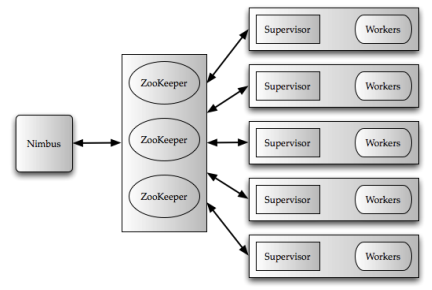
\includegraphics{figures/storm_cluster}
\caption{Storm architecture}
\label{figure:storm_cluster}
\end{figure}

All coordination between Nimbus and the Supervisors is done through a Zookeeper cluster. Additionally, the Nimbus daemon and Supervisor daemons are fail-fast and stateless, because all state is kept in Zookeeper or on local disk. This design leads to Storm clusters being incredibly stable, allowing the cluster to recover even if Nimbus or the Supervisors are killed and restarted afterwards.

\subsection{Topologies}

The core abstraction in Storm is the \emph{stream}, an unbounded sequence of tuples. A \emph{tuple} is a named list of values, and a field in a tuple can be an object of any type. The basic primitives Storm provides for doing stream transformations are spouts and bolts.

A \emph{spout} is a source of streams in a computation. Usually a spout reads from a queueing broker such as Kafka, but a spout can also generate its own stream or read from a streaming API.

A \emph{bolt} consumes any number of input streams, does some processing, and possibly emits new streams.  Most of the logic of a computation goes into bolts, such as functions, filters, streaming joins, streaming aggregations, databases queries, etc.

Networks of spouts and bolts are packaged into a topology which is the top-level abstraction is submitted to Storm clusters for execution. A \emph{topology} is a graph of stream transformations where each vertex is a spout or bolt. Edges in the graph indicate which bolts are subscribing to which streams. Topologies run indefinitely when deployed.

\begin{figure}[H]
\centering
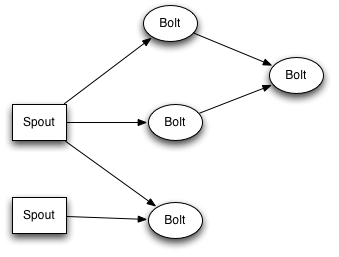
\includegraphics{figures/storm_topology}
\caption{Example storm topology}
\label{figure:storm_topology}
\end{figure}

Each component (spout or bolt) in a Storm topology executes in parallel. The degree of parallelism for each component can be configured and Storm will spawn that number of threads across the cluster to do the execution.

\subsection{Parallelism in Storm}

There are three main entities that are used to actually run a topology in a Storm cluster: worker processes, executors and tasks. The relationships between them are illustrated in Figure \ref{figure:storm_parallelism}.

\begin{figure}[H]
\centering
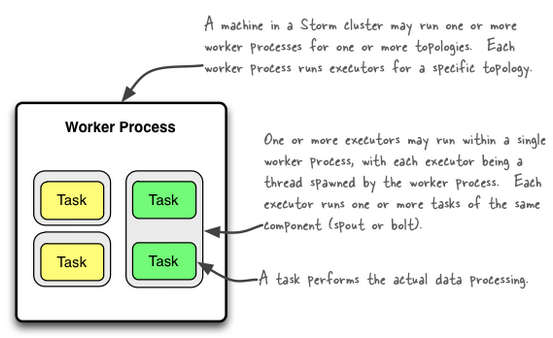
\includegraphics{figures/storm_parallelism}
\caption{The relationships between worker processes, executors and tasks}
\label{figure:storm_parallelism}
\end{figure}

A \emph{worker process} runs a JVM and executes a subset of a topology. Each worker process belongs to a specific topology and may run one or more executors.

An \emph{executor} is a thread spawned by a worker and may run one or more tasks for the same topology component. All of the tasks belonging to the same executor are run serially, since every executor always corresponds to one thread.

A \emph{task} performs the actual data processing for a topology component. Each spout or bolt is executed as many tasks across the cluster. The number of tasks for a component is static, in contrast to the number of executors for a component that can be changed after the topology has been started. By default, Storm will run one task per executor.

\subsection{Stream Groupings}

A \emph{stream grouping} defines how a stream between two components (spout to bolt or bolt to bolt) is partitioned among the tasks of each component. For example, the way tuples are emitted between the sets of tasks corresponding to Bolt A and Bolt B in Figure \ref{figure:storm_groupings} is defined by a stream grouping.

\begin{figure}[H]
\centering
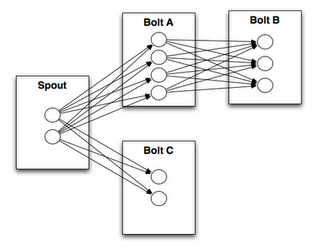
\includegraphics{figures/storm_groupings}
\caption{Task-level execution of a topology}
\label{figure:storm_groupings}
\end{figure}

Storm supports the following stream groupings:
\begin{itemize}
\item \textbf{Shuffle grouping:} Tuples are randomly and evenly distributed across the bolt's tasks.
\item \textbf{Fields grouping:} The stream is partitioned by the fields specified in the grouping. This guarantees that tuples with the same values on the specified fields are emitted to the same task.
\item \textbf{All grouping:} The stream is replicated across all the bolt's tasks.
\item \textbf{Global grouping:} The entire stream goes to a single one of the bolt's tasks.
\item \textbf{Local grouping:} If there are one or more of the bolt's tasks in the same worker process, tuples will be shuffled to just those in-process tasks.
\end{itemize}

\section{Hadoop Distibuted File System}

The Hadoop Distributed File System (HDFS) is a distributed file system designed to run on commodity hardware, inspired by the Google File System. It can reliably store very large files across machines in a large cluster and provides high throughput access to large data sets. HDFS is the storage part of the Hadoop framework, an Apache Top-Level Project since 2006.

Each file on HDFS is stored as a sequence of blocks of the same size, except the last block. Blocks belonging to a file are replicated for fault tolerance. The block size and replication factor are configurable per file.

HDFS has a master/slave architecture. An HDFS cluster consists of a single NameNode and one DataNode per node in the cluster. \emph{NameNode} is a master server that manages the file system namespace and regulates access to files by clients. Each \emph{DataNode} manages storage attached to the node that it run on. HDFS exposes a file system namespace and allows user data to be stored in files. Every file is split into blocks that are stored in a set of DataNodes. The NameNode determines the mapping of blocks to DataNodes and executes file system namespace operations like opening, closing, and renaming files and directories. The DataNodes are responsible for serving read and write requests from the file system’s clients and also perform block creation, deletion, and replication upon instruction from the NameNode.

\begin{figure}[H]
\centering
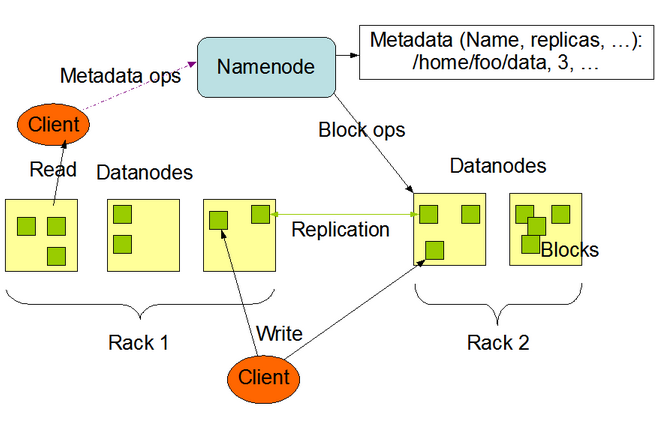
\includegraphics[width=1\textwidth]{figures/hdfs_architecture}
\caption{HDFS architecture}
\label{figure:hdfs_architecture}
\end{figure}

\section{HBase}
\subsection{Introduction}

HBase is a distributed non-relational database modeled after Google's BigTable, that runs on top of the HDFS. It provides a fault-tolerant way of storing large quantities of sparse data, while allowing random, real-time access to them. HBase is an Apache Top-Level Project since 2010.

HBase offers the following key features:
\begin{itemize}
\item \textbf{Linear and modular scalability:} HBase clusters expand by adding RegionServers that are hosted on commodity class servers, increasing storage and as well as processing capacity.
\item \textbf{Strictly consistent reads and writes:} HBase guarantees that all writes happen in an order, and all reads are seeing the most recent committed data.
\item \textbf{Automatic sharding of tables:} HBase tables are distributed on the cluster via regions, and regions are automatically split and re-distributed as data grows.
\item \textbf{Automatic failover support between RegionServers:} If a RegionServers fails, the regions it was hosting are reassigned between the available RegionServers.
\item \textbf{Integration with Hadoop MapReduce:} HBase supports massively parallelized processing via MapReduce for using HBase as both source and sink.
\item \textbf{Block Cache and Bloom Filters:} HBase supports a Block Cache and Bloom Filters for real-time queries.
\end{itemize}

\subsection{HBase Data Model}

The data model of HBase is very different from that of relational databases. As described in the  Bigtable paper, it is a sparse, distributed, persistent multidimensional sorted map. The map is indexed by a row key, column key, and a timestamp.

\begin{gather*}
(rowkey, column, timestamp) \rightarrow value
\end{gather*}

The basic elements of the HBase data model and the relations between them are presented below:
\begin{itemize}
\item \textbf{Table:} HBase organizes data into tables.
\item \textbf{Row:} Within a table, data is stored according to its row. A row consists of a row key and one or more columns with values associated with them. Rows are identified uniquely and sorted alphabetically by their row key.
\item \textbf{Column:} A column consists of a column family and a column qualifier, which are delimited by a : (colon) character.
\item \textbf{Column Family:} Data within a row is grouped by column family. Column families physically colocate a set of columns and their values. Each column family has a set of storage properties. For these reasons, column families must be declared up front at schema definition. Every row in a table has the same column families, though a given row might not store data in all of its families.
\item \textbf{Column Qualifier:} Data within a column family is addressed via its column
qualifier. Though column families are fixed at table creation, column qualifiers are mutable and may differ greatly between rows.
\item \textbf{Cell:} A combination of row, column family, and column qualifier uniquely identifies a cell. The data stored in a cell is that cell's value.
\item \textbf{Timestamp:} Values within a cell are versioned. A timestamp is written alongside each value, and is the identifier for a given version of a value.
\end{itemize}

\begin{figure}[H]
\centering
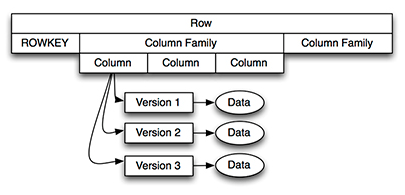
\includegraphics{figures/hbase_data_model}
\caption{HBase data model}
\label{figure:hbase_data_model}
\end{figure}

There are four primary data model operations in HBase:
\begin{itemize}
\item \textbf{Get:} Returns the values for a specified row.
\item \textbf{Put:} Adds a row to a table, if the key is new. If the key already exists, the row is updated.
\item \textbf{Scan:} Returns the values for a range of rows. Filters can also be used to narrow down the results.
\item \textbf{Delete:} Marks a row for deletion by adding a Tombstone marker. These rows are cleaned up during the next major compactions of the table.
\end{itemize}

\subsection{HBase Architecture}

In HBase, tables are are divided horizontally by row key range into \emph{Regions}. Regions are vertically divided by column families into \emph{Stores}, which are saved as files in HDFS (\emph{HFiles}). Figure \ref{figure:hbase_architecture} illustrates the architecture of HBase.

\begin{figure}[H]
\centering
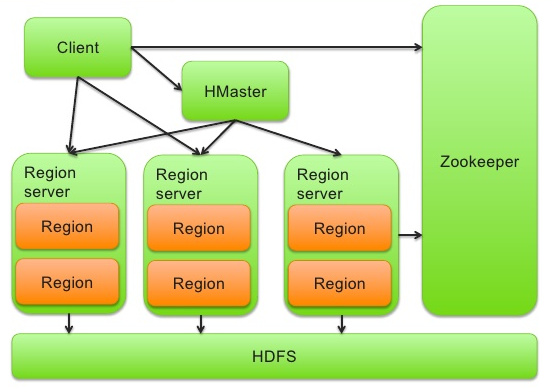
\includegraphics{figures/hbase_architecture}
\caption{HBase architecture}
\label{figure:hbase_architecture}
\end{figure}

An HBase cluster is composed of two types of servers in a master/slave type architecture. The \emph{HMaster} is responsible for monitoring all RegionServer instances in the cluster, and is the interface for all metadata changes. \emph{RegionServers} are responsible for serving and managing Regions. They are collocated with the HDFS DataNodes, which enables data locality for the data served by the RegionServers. HBase uses ZooKeeper as a distributed coordination service to maintain server state in the cluster. Zookeeper maintains which servers are alive and available, and provides server failure notification.

Every RegionServer has the following components:
\begin{itemize}
\item \textbf{WAL:} Write Ahead Log is used to store new data that hasn't yet been persisted to permanent storage. The WAL is used for recovery in the case of failure.
\item \textbf{BlockCache:} Keeps data blocks resident in memory after they are read. Least Recently Used data is evicted when full.
\item \textbf{MemStore:} Stores in-memory new data which has not yet been written to disk. There is one MemStore per column family per Region. Once the MemStore fills, its contents are written to disk as additional HFiles.
\item \textbf{Hfile:} Stores the rows as sorted key-values on disk.
\end{itemize}

\begin{figure}[H]
\centering
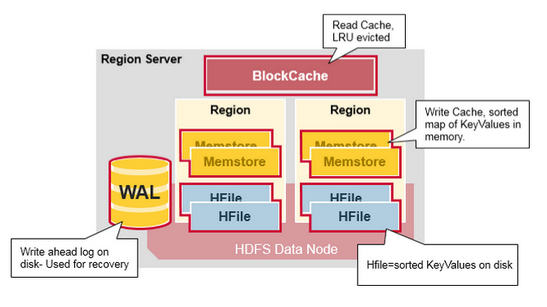
\includegraphics{figures/hbase_regionserver_components}
\caption{RegionServer components}
\label{figure:hbase_regionserver_components}
\end{figure}

\section{Phoenix}
\subsection{Introduction}

Apache Phoenix is relational database layer for HBase, targeting low latency queries over HBase data. Phoenix provides a JDBC driver that hides the intricacies of Hbase enabling users to create, delete, and alter SQL tables, views, indexes, and sequences, upsert and delete rows singly and in bulk and query data through SQL. Phoenix began as an internal project by the company Salesforce and was subsequently open-sourced and became a top-level Apache project on 2014.

\subsection{Phoenix Data Model}

The relational elements of the Phoenix data model are mapped to their respective counterparts in the HBase data model:

\begin{itemize}
\item A Phoenix table is mapped to an HBase table.
\item The Phoenix table's columns that are included in the primary key constraint are mapped together to the HBase row key.
\item The rest of the columns are mapped to HBase columns, consisting of a column family and a column qualifier.
\end{itemize}

Columns in a Phoenix table are assigned an SQL datatype. Phoenix serializes data from their datatype to byte arrays when upserting, because HBase stores everything as a byte array. In this way Phoenix allows typed access to HBase data.

\subsection{Phoenix Architecture}

On the client-side Phoenix is a JDBC driver that hides an HBase client from the user. The Phoenix driver compiles queries and other statements into native HBase client calls, enabling the building of low latency applications.

On the server-size a Phoenix jar is installed in every RegionServer, allowing Phoenix to take advantage of coprocessors and custom filters that HBase provides in order to increase performance. Coprocessors perform operations on the server-side thus minimizing client/server data transfer and custom filters prune data as close to the source as possible.

\begin{figure}[H]
\centering
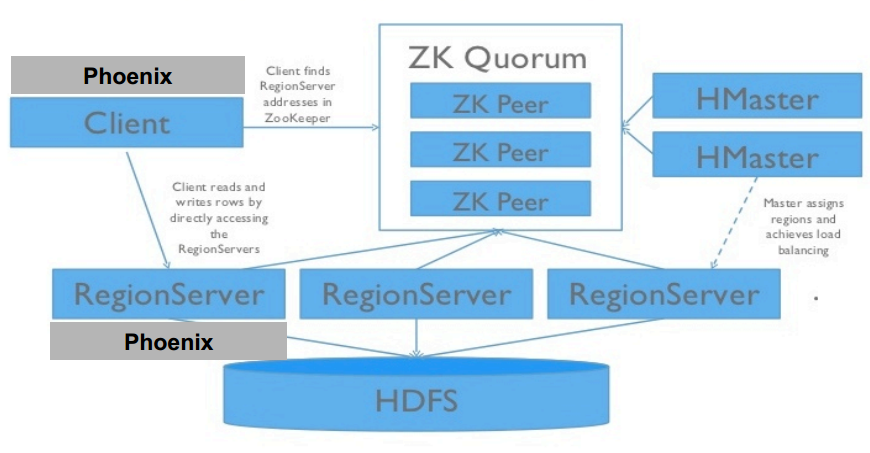
\includegraphics[width=1\textwidth]{figures/phoenix_architecture}
\caption{Phoenix and HBase architecture}
\label{figure:phoenix_architecture}
\end{figure}

\subsection{TopN Queries}

TopN queries return the top N rows, where top is determined by the ORDER BY clause and N is defined by the LIMIT clause of the SQL query. The execution of this query needs to make a pass through all the rows restricted by the WHERE clause and sort the results of the GROUP BY, which is very computationally expensive  for large tables. In order to decrease execution time, Phoenix handles these queries in a different way, using an approximate algorithm described below.

Firstly, the Phoenix client issues parallel scans restricted by the WHERE clause of the query. The parallel scans are \emph{chunked} by region boundaries and guideposts. \emph{Guideposts} are a set of keys per Region per column family collected by Phoenix at an equal byte distance from each other, that act as hints to improve the parallelization of queries on their Region. The rows that satisfy the WHERE clause are grouped for each chunk in parallel on the server-side by the TopN coprocessor, according to the GROUP BY clause. The TopN coprocessor of each RegionServer keeps only the top N rows for each chunk. Afterwards, the Phoenix client receives the top N rows for each chunk, does a final merge sort and returns the top N rows.

\cleardoublepage